\chapter{Úvod}
\label{sec:Introduction}

\begin{figure}[H]
\centering
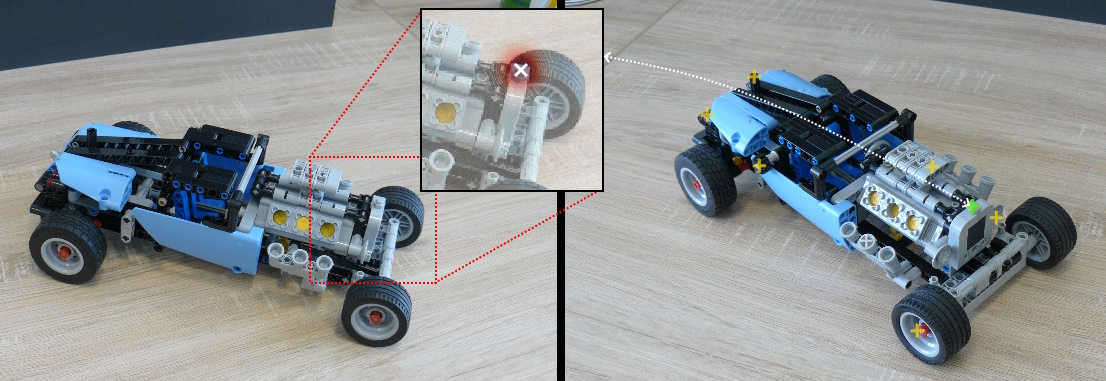
\includegraphics[width=1.0\textwidth,keepaspectratio]{Figures/bp_uvodni_obrazek.jpg}
\caption[Lokalizace klíčového bodu pro řešení PnP problému]{Lokalizace jednoho z klíčových bodů pro řešení PnP problému mezi reálným snímkem (vlevo) a syntetickým vykreslením (vpravo) se známými pozicemi klíčových bodů.}
\label{fig:bp_uvodni_obrazek}
\end{figure}


Lokalizace klíčových bodů zůstává nadále jedním z aktivně řešených problémů analýzy obrazu dnešní doby.
Klíčové body chápeme jako konkrétní body nacházející se na objektu zájmu, které chceme lokalizovat a následně sadu nalezených klíčových bodů použít pro další zpracování tykající se daného objektu zájmu či jeho částí.

Využití lokalizace bodů nacházíme kupříkladu při odhadu postoje osob \cite{humanpose}, v biomedicínské technice \cite{unet} nebo v rozšířené realitě (AR, ang. augmented reality) \cite{ar_pnp}.
Při lokalizaci musíme počítat s několika kvalitativně ovlivňujícími členy v obrazu jako např. natočení kamery, vzdálenost, osvětlení, zaostření a ostatní vlivy prostředí okolo klíčového bodu. Kvůli tomuto musí techniky pro lokalizaci klíčových bodů být invariantní vůči změnám ve scéně nebo vzhledu objektu.

Cílem této bakalářské práce je využít techniky lokalizace klíčových bodů pomocí hlubokých sítí U-Net (a jejími následovníky) pro zpřesnění odhadu 6 stupňů volnosti (DoF) transformace cílového objektu ve 3D prostoru pomocí PnP metod. PnP metody představují výpočetní techniky určené k řešení perspektivního problému n bodů, které se zaměřují na přesný odhad polohy a orientace 3D objektů na základě korespondence lokalizovaných klíčových bodů na 2D snímku a známých pozic klíčových bodů na 3D objektu.

Zde řešená úloha přesné lokalizace zvoleného klíčového bodu v předvybrané čtvercové oblasti celkového obrazu je ilustrována na obr. \ref{fig:bp_uvodni_obrazek}. Klíčový bod je pomocí hluboké konvoluční neuronové sítě korektně lokalizován na základě polohy maxima skalárního pole (pseudo)pravděpodobností. Klíčový bod také byl korektně klasifikován s třídou známého klíčového bodu. Za předpokladu korektní lokalizace co největšího počtu klíčových bodů můžeme polohu objektu z levé části snímku odhadnout pomocí zvolené PnP metody s využitím RANSAC techniky.

V rámci této práce byla nejprve v kapitole \ref{sec:Chapter2} provedena rešerše existujících přístupů pro lokalizaci (a popř. korespondenci) klíčových bodů. Rešerše začíná od počátků analýzy obrazu pro obdobné úlohy (jako je např. SIFT) přes hluboké učení několika variací sítí U-Net až po state-of-art přístupy jako je YOLOv8 či DINOv2. Detailně je popsán i modul STN, který slouží jako přídavný prvek řešící prostorovou invarianci do existujících sítí.

V kapitole \ref{sec:Chapter3} je představen dataset určen pro trénink našich neuronových sítích. Jsou představeny dostupné snímky, informace a korespondující CSV soubory ke snímkům. Popsány jsou také i některé detaily či poznatky týkající se datasetu. Následně v kapitole \ref{sec:Chapter4} jsou popsány zvolené přístupy pro lokalizaci klíčových bodů, což je v případě této práce síť U-Net, U-Net++ a zakomponování modulu STN. Součástí jsou všechny detaily týkající se architektur implementovaných neuronových sítí, návrh ztrátové funkce, použití datasetu, augmentace dat a dalších relevantních částí. Následuje kapitola \ref{sec:Chapter5}, kde jsou popsány detaily implementace pomocí knihovny TensorFlow 2. Popsána je příprava, průběh tréninků a také i zajímavé části implementace ztrátové funkce a modulu STN.

V kapitole \ref{sec:Chapter6} jsou popsány výsledky, evaluace, experimenty a dedukce plynoucí z výsledků praktických úloh provedených v rámci této práce. Součástí je i samostatný experiment pomocí sítě DINOv2 od Meta AI. V kapitole \ref{sec:Chapter7} jsou popsány finální závěry a myšlenky plynoucí ze zjištění v této práci.
\endinput